\documentclass{beamer}

\usetheme{Warsaw}
\usecolortheme{seahorse}
\setbeamertemplate{navigation symbols}{}
\setbeamertemplate{bibliography item}{\insertbiblabel}
\setbeamercolor{background canvas}{bg=}
\usepackage{beamerthemesplit}
\usepackage{pgf}
\usepackage{epsfig}
\usepackage{epstopdf}
\usepackage{graphicx}
\usepackage{slashbox}
\usepackage{url}
\usepackage{listings}
\usepackage{polski}
\usepackage[utf8]{inputenc}
\usepackage[absolute,overlay]{textpos}
\usepackage{graphicx}
\newcommand{\IR}{\bbold R}
\def\Rset{\mathbb{R}}
\def\Zset{\mathbb{Z}}
\newcommand{\refbr}[1]{(\ref{#1})}
\newcommand{\beq}{\begin{equation}}
\newcommand{\eeq}{\end{equation}}
\newcommand{\und}[1]{\underline{#1}}
\newcommand\pro{\item[$+$]}
\newcommand\con{\item[$-$]}
\newcounter{saveenumi}
\newcommand{\seti}{\setcounter{saveenumi}{\value{enumi}}}
\newcommand{\conti}{\setcounter{enumi}{\value{saveenumi}}}

\hypersetup{
   pdftitle={Oprogramowanie do gier opartych o planszę w postaci szachownicy},
   pdfauthor={Jakub Ostrzołek},
   pdfborder={0 0 0}
}

\title[Silnik gier opartych o szachownicę \insertframenumber/\inserttotalframenumber]{
   Projekt i wykonanie oprogramowania do gier planszowych opartych
   o planszę postaci szachownicy -- podejście w oparciu o dedykowany
   język dziedzinowy.}
\author[Jakub Ostrzołek]{\textbf{Jakub Ostrzołek} \\%
\footnotesize Promotor: dr inż. Patryk Chaber}
\institute{Instytut Automatyki i Technik Informacyjnych\\%
Politechnika Warszawska}

\begin{document}

\frame{\titlepage}

\frame{\tableofcontents\frametitle{Plan prezentacji}}

\section{Cel pracy}
\begin{frame}
	\frametitle{Cel pracy}
	3 główne cele pracy:
	\begin{enumerate}
		\item opracowanie języka DSL\footnotemark do opisywania zasad gier planszowych opartych o szachownicę
		\item implementacja silnika gry
		      \begin{itemize}
			      \item potrafi interpretować zasady w ww. języku
			      \item pozwala na rozgrywkę dwóch osób
		      \end{itemize}
		\item stworzenie interfejsu użytkownika
	\end{enumerate}
	\footnotetext{DSL (ang. Domain Specific Language) - język dziedzinowy}
\end{frame}

\section{Tematyka pracy}

\begin{frame}
	\frametitle{Język - wstępne założenia}
	\begin{itemize}
		\item Składnia języka jest kluczowym elementem rozwiązania
		\item Wstępne założenia:
		      \begin{itemize}
			      \item pozwala wyrazić zasady min. 3 rodzajów  gier
			      \item możliwie nieskomplikowany
			      \item ograniczony do 2-osobowych gier opartych o szachownicę
			      \item zwięzły
			      \item wymaga rozumienia podstawowych zasad programowania
		      \end{itemize}
	\end{itemize}
\end{frame}

\begin{frame}
	\frametitle{Język - elementy}
	Elementy języka:
	\begin{itemize}
		\item definicja planszy (rozmiar)
		\item typy figur
		      \begin{itemize}
			      \item generatory ruchu (funkcje typu: {\tt pozycja $\rightarrow$ []pozycja})
			      \item akcje (funkcje typu: {\tt pozycja $\rightarrow$ void})
		      \end{itemize}
		\item walidatory stanu gry po ruchu (funkcje typu: {\tt ruch $\rightarrow$ bool})
		\item stan początkowy -- ustawienie figur
		\item predykat zakończenia gry + wybór zwycięzcy
		\item funkcja przebiegu rundy
	\end{itemize}
\end{frame}

\begin{frame}[allowframebreaks]
	\frametitle{Język - podejścia}
	Możliwe podejścia:
	\begin{enumerate}
		\item Stworzenie własnego języka DSL
		      \begin{itemize}
			      \pro całkowita możliwość dostosowania języka do potrzeb
			      \con tworzenie parsera bardzo pracochłonne
			      \con brak dodatkowych narzędzi (formatowanie, detekcja błędów składniowych, itp.)
			      \con brak znajomości języka u użytkowników
		      \end{itemize}
		\item Stworzenie DSL zanurzonego w języku programowania (np. Kotlin, Haskell, Lua)
		      \begin{itemize}
			      \pro dostępne wszystkie możliwości języka nadrzędnego
			      \pro znajoma składnia dla użytkowników
			      \con trudny do ograniczenia (problem bezpieczeństwa)
		      \end{itemize}
		\framebreak
		\item Użycie istniejącego formatu (np. {\tt JSON}, {\tt YAML})
		      \begin{itemize}
			      \pro formaty popularne i znane przez użytkowników
			      \pro brak potrzeby tworzenia parsera
			      \con brak łatwego zapisu wyrażeń, funkcji, pętli, itp.
			      \con brak możliwości modyfikacji składni języka
		      \end{itemize}
	\end{enumerate}
\end{frame}

\begin{frame}[t]
	\vspace{0.7cm}
	\frametitle{Silnik gry}
	Silnik gry -- maszyna stanów
	\begin{itemize}
		\item dla każdego stanu generuje możliwe przejścia
		\item odseparowany od modułu parsera języka
		\item dobrze przetestowany
	\end{itemize}
	\begin{textblock*}{5cm}(7.5cm,4.5cm)
		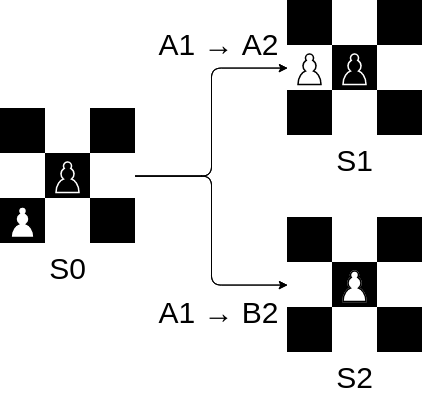
\includegraphics[width=4.5cm]{stany.png}
	\end{textblock*}
\end{frame}

\begin{frame}
	\frametitle{Interfejs użytkownika}
	\begin{itemize}
		\item Tematycznie najmniej istotna część projektu
		\item Wersja minimalna
		      \begin{itemize}
			      \item interfejs terminalowy
			      \item rozgrywka na jednym urządzeniu
		      \end{itemize}
		\item Wersja docelowa
		      \begin{itemize}
			      \item interfejs w przeglądarce internetowej
			      \item komunikacja z serwerem, na którym działa silnik gry (po protokole HTTP/WS)
			      \item rozgrywka poprzez 2 urządzenia
		      \end{itemize}
	\end{itemize}
\end{frame}


\section{Istniejące rozwiązania}

\begin{frame}
	\frametitle{BGD -- BoardGameDescription\cite{BGD}}
	\begin{itemize}
		\item Język opisu gier planszowych (szeroki zakres)
		\item Główny cel: możliwość opisu jak największej liczby gier
		\item Opis gry za pomocą abstrakcyjnych elementów składowych (np. obiekt, lokacja, widoczność)
		\item Mało zwięzły (np. implementacja Chińczyka - 400 linii, Manilla - 1100 linii)
		\item Brak udogodnień znanych z języków programowania (np. pętle, listy)
	\end{itemize}
\end{frame}

\begin{frame}
	\frametitle{RAS -- Rule Automation System\cite{RAS}}
	\begin{itemize}
		\item Język opisu gier karcianych
		\item Główny cel: używanie przez ludzi niezaznajomionych z programowaniem
		\item Ograniczony tylko do gier karcianych
		\item Brak udogodnień znanych z języków programowania (np. pętle, listy)
	\end{itemize}
\end{frame}

\begin{frame}
	\frametitle{Metagame\cite{metagame}}
	\begin{itemize}
		\item Język opisu gier opartych o szachownicę
		\item Główny cel: dokładny opis gier na potrzeby zadań SI
		\item Bardzo rozbudowany, zawiera informacje przydatne do uczenia modelów SI
		\item Skomplikowany w pisaniu i rozumieniu
	\end{itemize}
\end{frame}

\begin{frame}
	\frametitle{GDL -- Game Description Language\cite{GDL}}
	\begin{itemize}
		\item Język opisu gier planszowych (szeroki zakres)
		\item Główny cel: opis jak największej liczby gier przy pomocy prostej składni
		\item Podobny do Prologa -- predykaty głównym budulcem zasad
		\item Bardzo elastyczny, przy tym mało skomplikowany
		\item Brak wbudowanych konceptów gier planszowych (takich jak: plansza, gracz)
		\item Brak wbudowanych operacji arytmetycznych
	\end{itemize}
\end{frame}

\section{Zadania pracy}

\begin{frame}
	\frametitle{Język -- wybór podejścia}
	Istniejący format danych HCL jako baza języka
	\begin{itemize}
		\item sprawdzony format używany m. in. w Terraformie\footnotemark
		\item zawiera elementy standardowych języków programowania:
		      \begin{itemize}
			      \item ewaluacja wyrażeń arytmetycznych i logicznych
			      \item wykonywanie funkcji zdefiniowanych w kontekście ewaluacji
			      \item pętle w postaci list/dictionary comprehensions
		      \end{itemize}
		\item oficjalny dodatek {\tt userfunc} umożliwia definicję funkcji przez użytkownika
		\item zwięzły i czytelny kod
	\end{itemize}
	\footnotetext{Terraform -- narzędzie do zarządzania infrastrukturą komputerową w modelu infrastruktura jako kod (ang. IaC - Infrastructure as Code)}
\end{frame}

\begin{frame}
	\frametitle{Język -- przykładowy kod}
	Istniejący format danych HCL jako baza języka
	\begin{itemize}
		\item sprawdzony format używany m. in. w Terraformie\footnotemark
		\item zawiera elementy standardowych języków programowania:
		      \begin{itemize}
			      \item ewaluacja wyrażeń arytmetycznych i logicznych
			      \item wykonywanie funkcji zdefiniowanych w kontekście ewaluacji
			      \item pętle w postaci list/dictionary comprehensions
		      \end{itemize}
		\item oficjalny dodatek {\tt userfunc} umożliwia definicję funkcji przez użytkownika
		\item zwięzły i czytelny kod
	\end{itemize}
	\footnotetext{Terraform -- narzędzie do zarządzania infrastrukturą komputerową w modelu infrastruktura jako kod (ang. IaC - Infrastructure as Code)}
\end{frame}

\section{Dotychczasowe wyniki pracy}

\section{Plan przyszłych prac}

\begin{frame}[allowframebreaks]
	\frametitle{Bibliografia}
	\bibliographystyle{plain}
	\begin{thebibliography}{9}
		\bibitem{BGD} P. Schroten. "Introducing BGD: a DSL to express board games and gameplay" (2019).

		\bibitem{RAS} V. Lap. "Introducing RAS: A Domain Specific Language For Trading Card Games" (2018).

		\bibitem{metagame}  B. Pell. "METAGAME: A New Challenge for Games and Learning. In Heuristic Programming in Artificial Intelligence: The Third Computer Olympiad." (1992).

		\bibitem{GDL}  N. Love, T. Hinrichs, D. Haley, E. Schkufza, and M. Genesereth. "General Game Playing:
Game Description Language Specification. Technical report, Stanford Logic Group" (2006).

		\bibitem{GGP} Kowalski, Jakub. "General Game Description Languages" (2016).
	\end{thebibliography}
\end{frame}

\end{document}
